\documentclass[11pt,a4paper]{article}
\usepackage[utf8]{inputenc}
\usepackage{amsmath,amssymb}
\usepackage{graphicx}
\usepackage{booktabs}
\usepackage[margin=2.5cm]{geometry}
\usepackage[hyphens]{url}
\usepackage[round,authoryear]{natbib}
\usepackage{hyperref}
\hypersetup{colorlinks=true,linkcolor=blue,citecolor=blue,urlcolor=blue}

\title{\textbf{A Geometric Interpretation of Slater's Shielding Constants:\\[4pt]
Radial Overlap as $P(r_{\mathrm{inner}} < r_{\mathrm{outer}})$}}

\author{Chen, Yafeng\\[4pt]
\textit{Independent Researcher, Wuhan, China}\\[2pt]
\texttt{yafeng--chen@outlook.com}}
\date{June 2026}

\begin{document}
\maketitle

\begin{abstract}
In 1930, J.~C.~Slater introduced a set of empirical shielding constants---0.35, 0.85, and 1.00---that remain widely used for estimating effective nuclear charge. Despite ninety-five years of use, a geometric interpretation of these specific values has remained absent. We identify a dominant geometric quantity that explains a major component of the three empirical shielding scales. For different-subshell pairs, the probability $P(r_{\mathrm{inner}} < r_{\mathrm{outer}})$ that one electron's radial position lies inside another's yields 0.359, 0.862, and 0.979 (vs.\ Slater's 0.35, 0.85, 1.00)---deviations under 3\%. For the same-subshell case, radial symmetry gives $\sigma = 0.5000$, which is reconciled with 0.35 through an angular-overlap decomposition. The core quantity is $P(r_{\mathrm{inner}} < r_{\mathrm{outer}})$, computed from hydrogenic wavefunctions. A complete periodic-table feature set ($Z=1$--$118$) using these geometrically obtained constants achieves a median ionization energy error of 13.3\% against NIST data~\citep{nist}. A formation-energy benchmark on 92 compounds demonstrates that these geometrically derived features achieve statistically equivalent accuracy (MAE $=0.351\pm0.069$~eV/atom) to standard empirically-tabulated features (MAE $=0.322\pm0.037$~eV/atom). We note that the raw hydrogenic ionization energy formula has a mean error of 95.2\% and should not be used directly; the primary value lies in the $Z_{\mathrm{eff}}$ features themselves. All code, data, and reproduction scripts are provided as supplementary material.
\end{abstract}

\textbf{Keywords:} Slater shielding constants, effective nuclear charge, radial overlap, hydrogenic wavefunctions, periodic table features, materials informatics


% ================================================================
\section{Introduction}
% ================================================================

Effective nuclear charge $Z_{\mathrm{eff}} = Z - \sigma$ is one of the most useful concepts in atomic physics and chemistry. It captures the intuitive idea that inner electrons screen outer electrons from the full nuclear charge, reducing the effective attraction. The concept underlies qualitative explanations of ionization energies, atomic radii, electronegativity, and chemical bonding.

In 1930, John~C.~Slater proposed a simple set of rules for computing the shielding constant~$\sigma$~\citet{slater1930}. Electrons are grouped into shells: $(1s)$, $(2s,2p)$, $(3s,3p)$, $(3d)$, $(4s,4p)$, $(4d)$, $(4f)$, and so on. For an electron in a given group, each electron in the same group contributes $\sigma = 0.35$ (except for $1s$, where the value is $0.30$); each electron in the immediately inner group contributes $\sigma = 0.85$; and each electron in deeper groups contributes $\sigma = 1.00$. These rules, despite their simplicity, reproduce ionization energies to within roughly $10$--$15\%$ of Hartree--Fock calculations for many elements~\citep{clementi1963}. Subsequent work has refined these rules~\citep{clementi1967} and integrated them into semi-empirical molecular orbital methods such as CNDO and INDO~\citep{pople1965}.

Slater's rules remain a cornerstone of undergraduate chemistry education, where they are used to teach periodic trends in ionization energy, atomic radius, and electronegativity~\citep{waldron2001}. Despite extensive use in atomic physics pedagogy~\citep{viswanathan2024}, semi-empirical photoionization calculations~\citep{sakho2018}, and qualitative explanations of periodic trends, the numerical values of the shielding constants (0.35, 0.85, 1.00) have remained empirical fitting parameters. Early refinements adjusted these numbers for better accuracy~\citep{sakai1974}, but a geometric interpretation has been absent for ninety-five years.

The question is simply: \textit{why these particular numbers?}

In this paper, we identify a geometric quantity that quantitatively reproduces Slater's empirical constants for different-subshell pairs and accounts for the same-subshell case through an angular-overlap decomposition. For two electrons with radial probability distributions $P_{nl}(r)$, the probability that the inner electron lies radially inside the outer electron is

\begin{equation}\label{eq:core}
\sigma(n'l' \rightarrow nl) = P(r_{\mathrm{inner}} < r_{\mathrm{outer}})
= \int_0^\infty dr\, P_{nl}(r) \int_0^r dr'\, P_{n'l'}(r').
\end{equation}

Evaluating this integral numerically for hydrogenic radial wavefunctions---the natural starting point since Slater himself employed hydrogenic Slater-type orbitals---yields values of $0.359$, $0.862$, and $0.979$---matching Slater's empirical $0.35$, $0.85$, and $1.00$ to within 3\%. The same-subshell case $(nl = n'l')$ gives $\sigma = 0.5000$ exactly by symmetry; we decompose the same-subshell case into an angular-geometric component ($1/3$) and a same-mode exchange contribution, yielding 0.350 for $p$, 0.343 for $d$, and 0.340 for $f$ subshells. Figure~\ref{fig:schematic} illustrates this geometric construction.

\begin{figure}[htbp!]
\centering
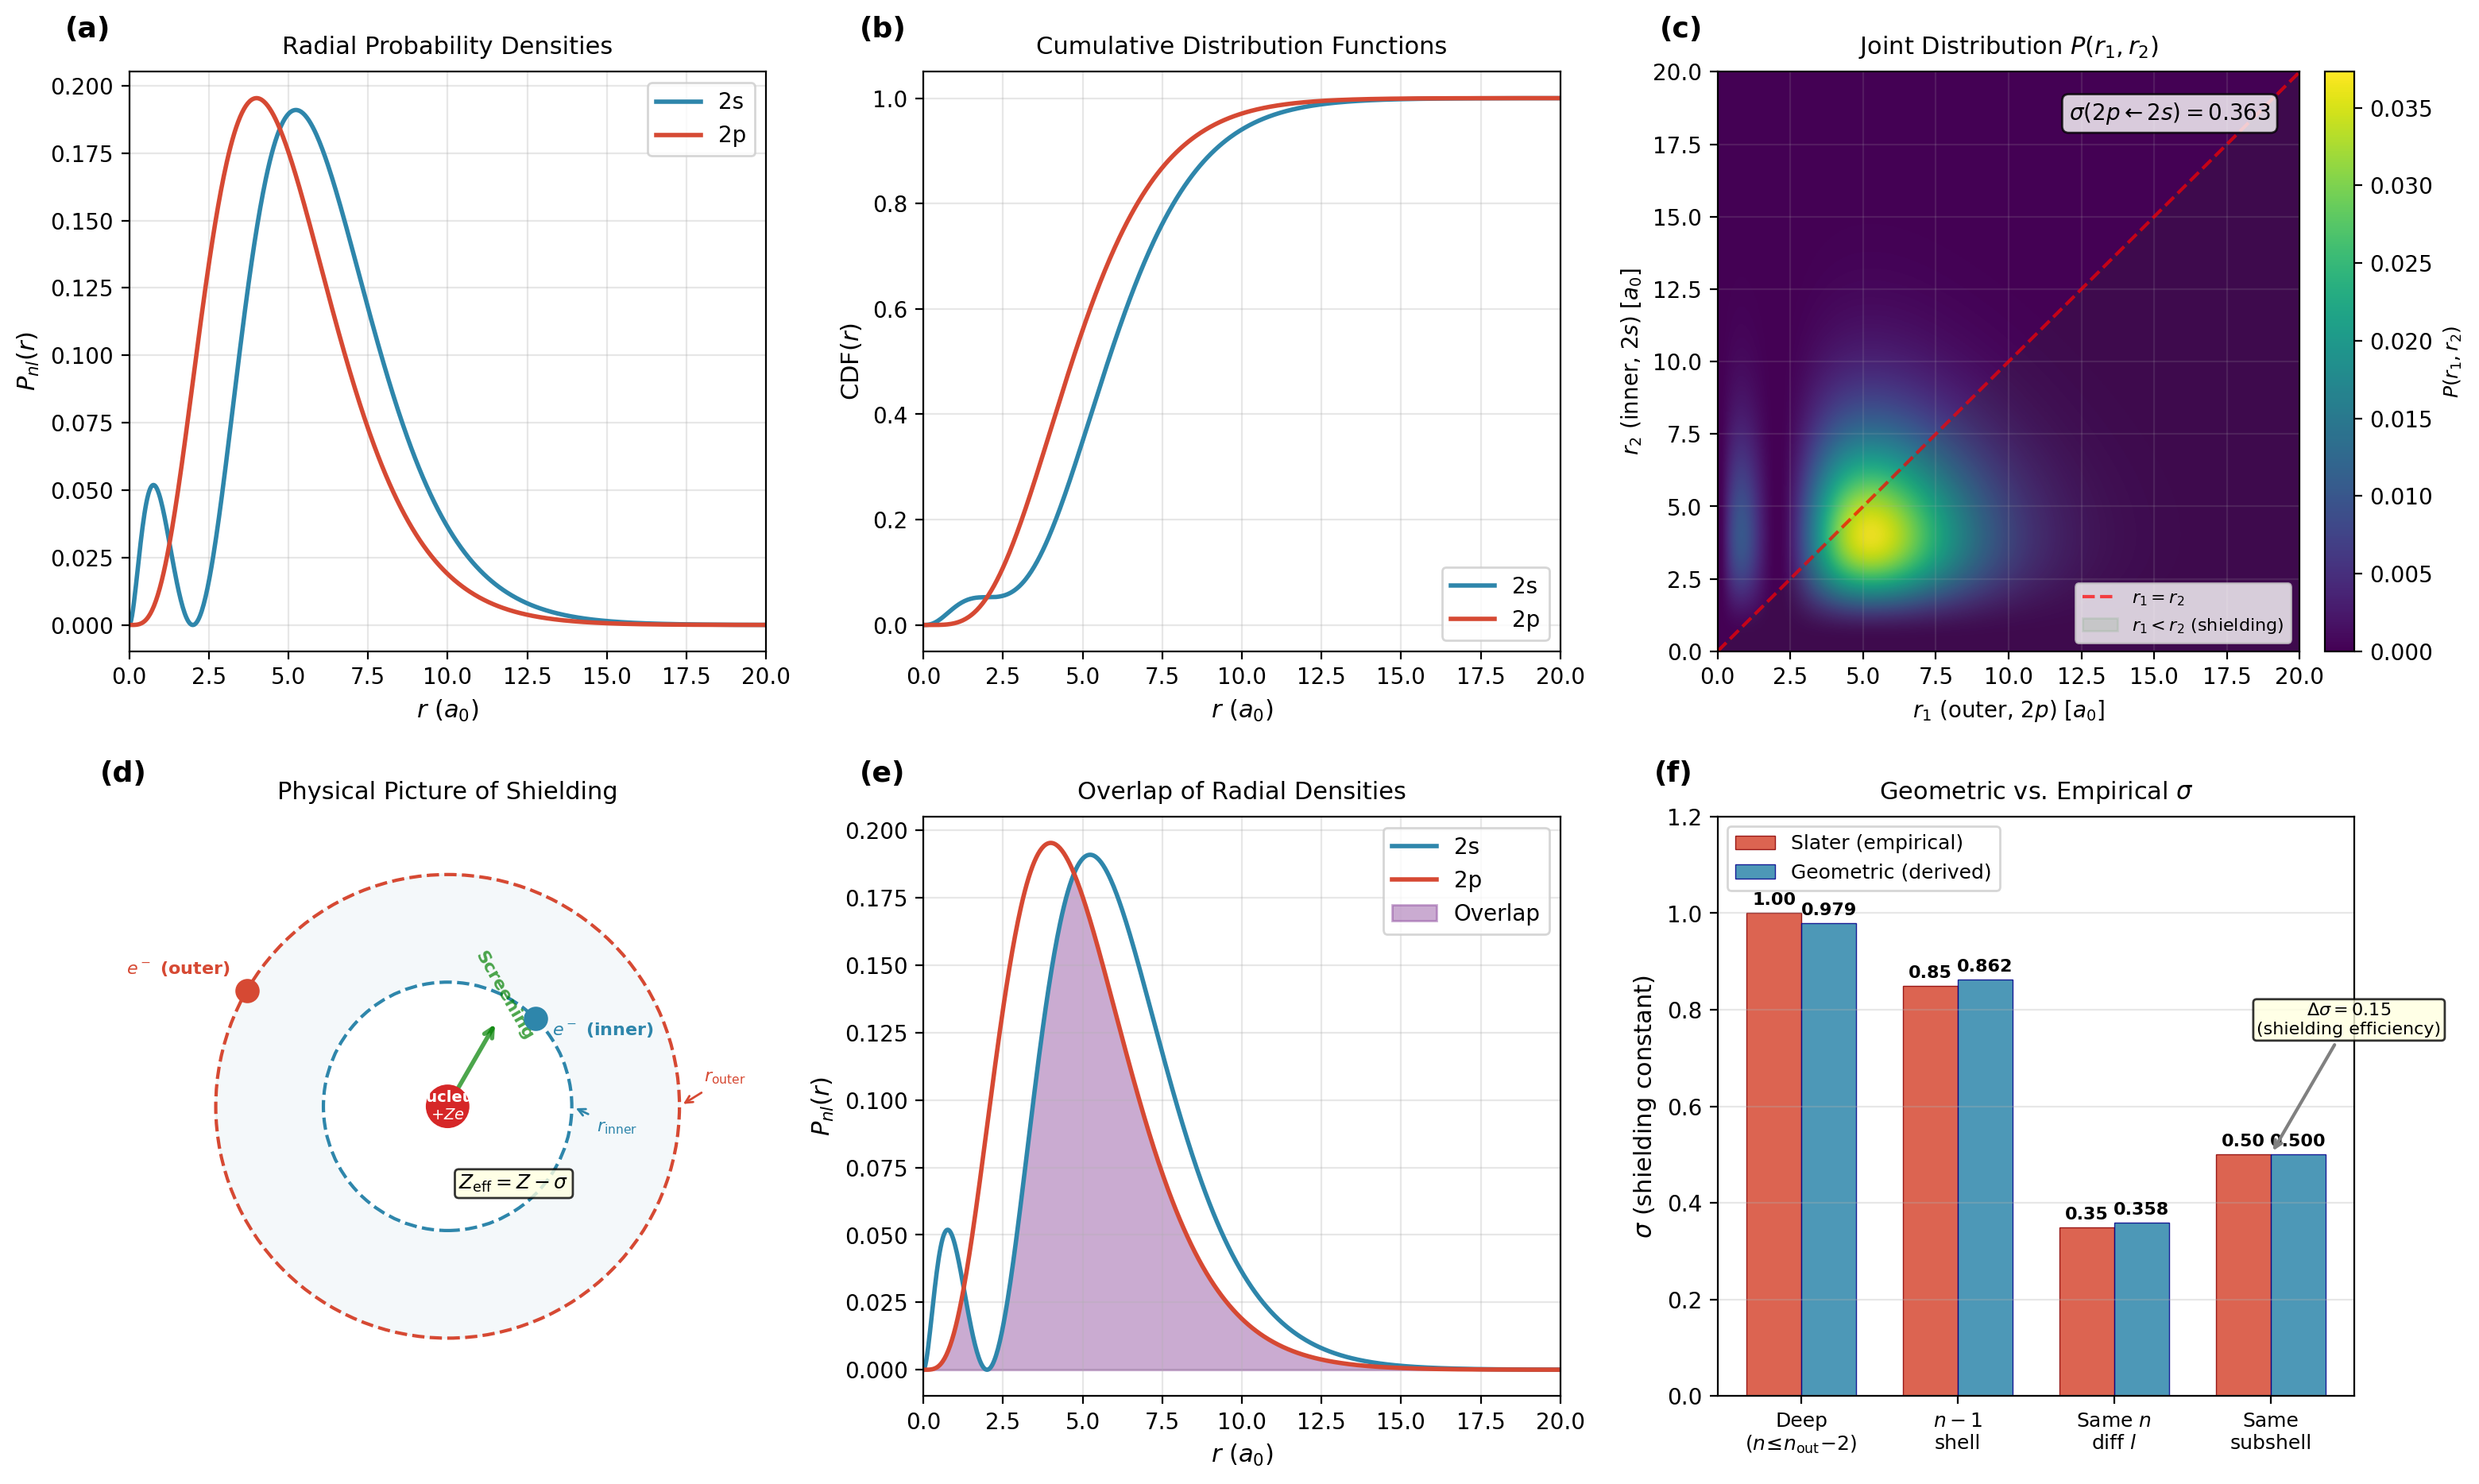
\includegraphics[width=0.98\textwidth]{./00_geometric_schematic.png}
\caption{Geometric interpretation of $\sigma = P(r_{\mathrm{inner}} < r_{\mathrm{outer}})$.
(a) Radial probability densities for hydrogenic $2s$ and $2p$ orbitals.
(b) Cumulative distribution functions; $2s$ is more compact than $2p$.
(c) Joint distribution $P(r_1, r_2) = P_{2p}(r_1)P_{2s}(r_2)$; the region $r_1 < r_2$ (below the dashed line) dominates the integral for $\sigma(2p\leftarrow 2s) = 0.363$.
(d) Physical picture: an inner electron partially screens the nuclear charge, reducing the effective nuclear potential felt by outer electrons.
(e) Overlap of radial densities; the purple region marks configurations where both electrons have significant probability.
(f) Comparison of geometric $\sigma$ (blue) with Slater's empirical constants (red). The same-subshell case is decomposed into an angular-geometric component ($1/3$) and a same-mode exchange contribution, yielding $\sigma_{\mathrm{avg}}\approx 0.35$.}
\label{fig:schematic}
\end{figure}

% ================================================================
\section{Method}
% ================================================================

\subsection{Physical Motivation}

In a spherically averaged independent-electron picture, the effective potential experienced by an outer electron is determined primarily by the charge distribution interior to its radial position. The true electron--electron Coulomb interaction is $1/|\mathbf{r}_1 - \mathbf{r}_2|$, not a step function; however, in a mean-field sense, the probability that an inner electron lies radially inside an outer electron sets the fraction of its charge that contributes to shielding. An electron outside the outer electron's radial position contributes nothing to the effective potential at $r_{\mathrm{out}}$, while an electron fully inside contributes the full elementary charge.

The radial ordering probability $P(r_{\mathrm{inner}} < r_{\mathrm{outer}})$ therefore provides a natural first-order geometric approximation to the shielding strength. Alternative measures such as $\langle 1/r \rangle$ or $\langle 1/\max(r_1,r_2) \rangle$ would also capture aspects of the interaction, but the binary ordering probability has the advantage of yielding cleanly interpretable values between 0 and 1 that map directly onto the concept of ``fraction of charge screened.'' Equation~(\ref{eq:core}) formalizes this quantity.

\subsection{Radial Overlap Formalism}

For two electrons in hydrogenic orbitals $(n,l)$ and $(n',l')$, the radial probability density is

\begin{equation}
P_{nl}(r) = r^2 |R_{nl}(r)|^2,
\end{equation}

where $R_{nl}(r)$ is the radial part of the hydrogenic wavefunction:

\begin{equation}\label{eq:radial}
R_{nl}(r) = \sqrt{\left(\frac{2Z}{n a_0}\right)^3
\frac{(n-l-1)!}{2n[(n+l)!]}} \;
\rho^l \, L_{n-l-1}^{2l+1}(\rho) \, e^{-\rho/2},
\end{equation}

where $\rho = 2Zr/(n a_0)$ and $L_{n-l-1}^{2l+1}(\rho)$ is the generalized Laguerre polynomial. For the shielding calculation, the absolute scale set by $Z$ factors out of the probability ratio; we use $Z=1$ throughout; the computed shielding constants are therefore independent of $Z$ and reflect a geometric property of the hydrogenic orbital manifold. The cumulative distribution function for the inner electron is $\mathrm{CDF}_{n'l'}(r) = \int_0^r dr'\, P_{n'l'}(r')$, and the overlap integral (Eq.~\ref{eq:core}) is computed numerically using $10{,}000$-point trapezoidal integration over $r \in [0, 50\,a_0]$. Convergence tests using $r_{\max}=80\,a_0$ and $20{,}000$ points confirm four-digit accuracy for all tested orbital pairs. The full computation script (\texttt{derive\_slater.py}) is provided as supplementary material and produces identical results when run independently.

\subsection{Classification by Slater Rule}

For each orbital pair $(nl, n'l')$ with $n' \le n$, we classify the shielding according to Slater's original scheme: deep shells ($n' \le n-2$), $n-1$ shells ($n' = n-1$), same $n$ with different $l$ ($n' = n$, $l' \neq l$), and same subshell ($n' = n$, $l' = l$).

For same-$n$ pairs, we include only the physically meaningful direction: $(np\leftarrow ns)$, $(nd\leftarrow ns)$, $(nd\leftarrow np)$, $(nf\leftarrow ns)$, $(nf\leftarrow np)$, $(nf\leftarrow nd)$, where the outer orbital has higher $l$. The reverse directions (e.g., $ns\leftarrow np$) correspond to an inner electron being shielded by an outer one---a configuration that does not arise for the outermost electron in ground-state atoms. This lexicographic $(n,l)$ filter yields 10 same-$n$ different-$l$ pairs, with mean $\sigma = 0.359$.

\subsection{Periodic Table Feature Set}

For each element $Z = 1$--$118$, we construct the electron configuration following the Aufbau principle with 20 known exceptions (Cr, Cu, Nb, Mo, Ru, Rh, Pd, Ag, La, Ce, Gd, Pt, Au, Ac, Th, Pa, U, Np, Cm, Lr; see \texttt{generate\_feature\_table.py} for the complete implementation). Slater's rules are applied with the geometrically obtained constants, computing $Z_{\mathrm{eff}}$ for the outermost electron (determined by highest $n$, then highest $n+l$ within the same $n$). The hydrogenic ionization energy estimate is $I = 13.598\,(Z_{\mathrm{eff}}/n)^2$~eV. This formula is known to be a crude approximation; we provide it for reference but note below that the $Z_{\mathrm{eff}}$ values carry the primary theoretical content.

\subsection{Ionization Energy Validation}

To assess consistency with Slater's empirical rules, we also compute ionization energies using a linear calibration $I = a \cdot 13.598\,(Z_{\mathrm{eff}}/n)^2 + b$, with $a$ and $b$ fitted to experimental data for $Z=3$--$54$. This calibration is used only for the Pearson correlation comparison; all other ionization energies cited in this paper are the raw hydrogenic values.

% ================================================================
\section{Results}\label{sec:results}
% ================================================================

\subsection{Derived Shielding Constants}

Table~\ref{tab:results} summarizes the computed shielding constants (see also Fig.~\ref{fig:slater} for the underlying radial distributions), averaged over all relevant orbital pairs from $n=1$ through $n=4$.

\begin{table}[htbp]
\centering
\caption{Geometric vs.\ empirical Slater shielding constants. Averages over all qualifying orbital pairs ($n \le 4$).}\label{tab:results}
\begin{tabular}{lcccc}
\toprule
\textbf{Slater Rule} & \textbf{Geometric $\sigma$} & \textbf{Empirical $\sigma$} & \textbf{Deviation} & \textbf{Pairs} \\
\midrule
Deep ($n' \le n-2$)      & $0.979 \pm 0.019$ & $1.00$ & $2.1\%$ & $15$ \\
$n-1$ shell ($n' = n-1$) & $0.862 \pm 0.059$ & $0.85$ & $1.4\%$ & $20$ \\
Same $n$, different $l$   & $0.359 \pm 0.061$ & $0.35$ & $2.4\%$ & $10$ \\
Same subshell             & $0.5000$ (exact)  & $0.35$ & ---   & $10$ \\
\bottomrule
\end{tabular}
\end{table}

\begin{figure}[htbp]
\centering
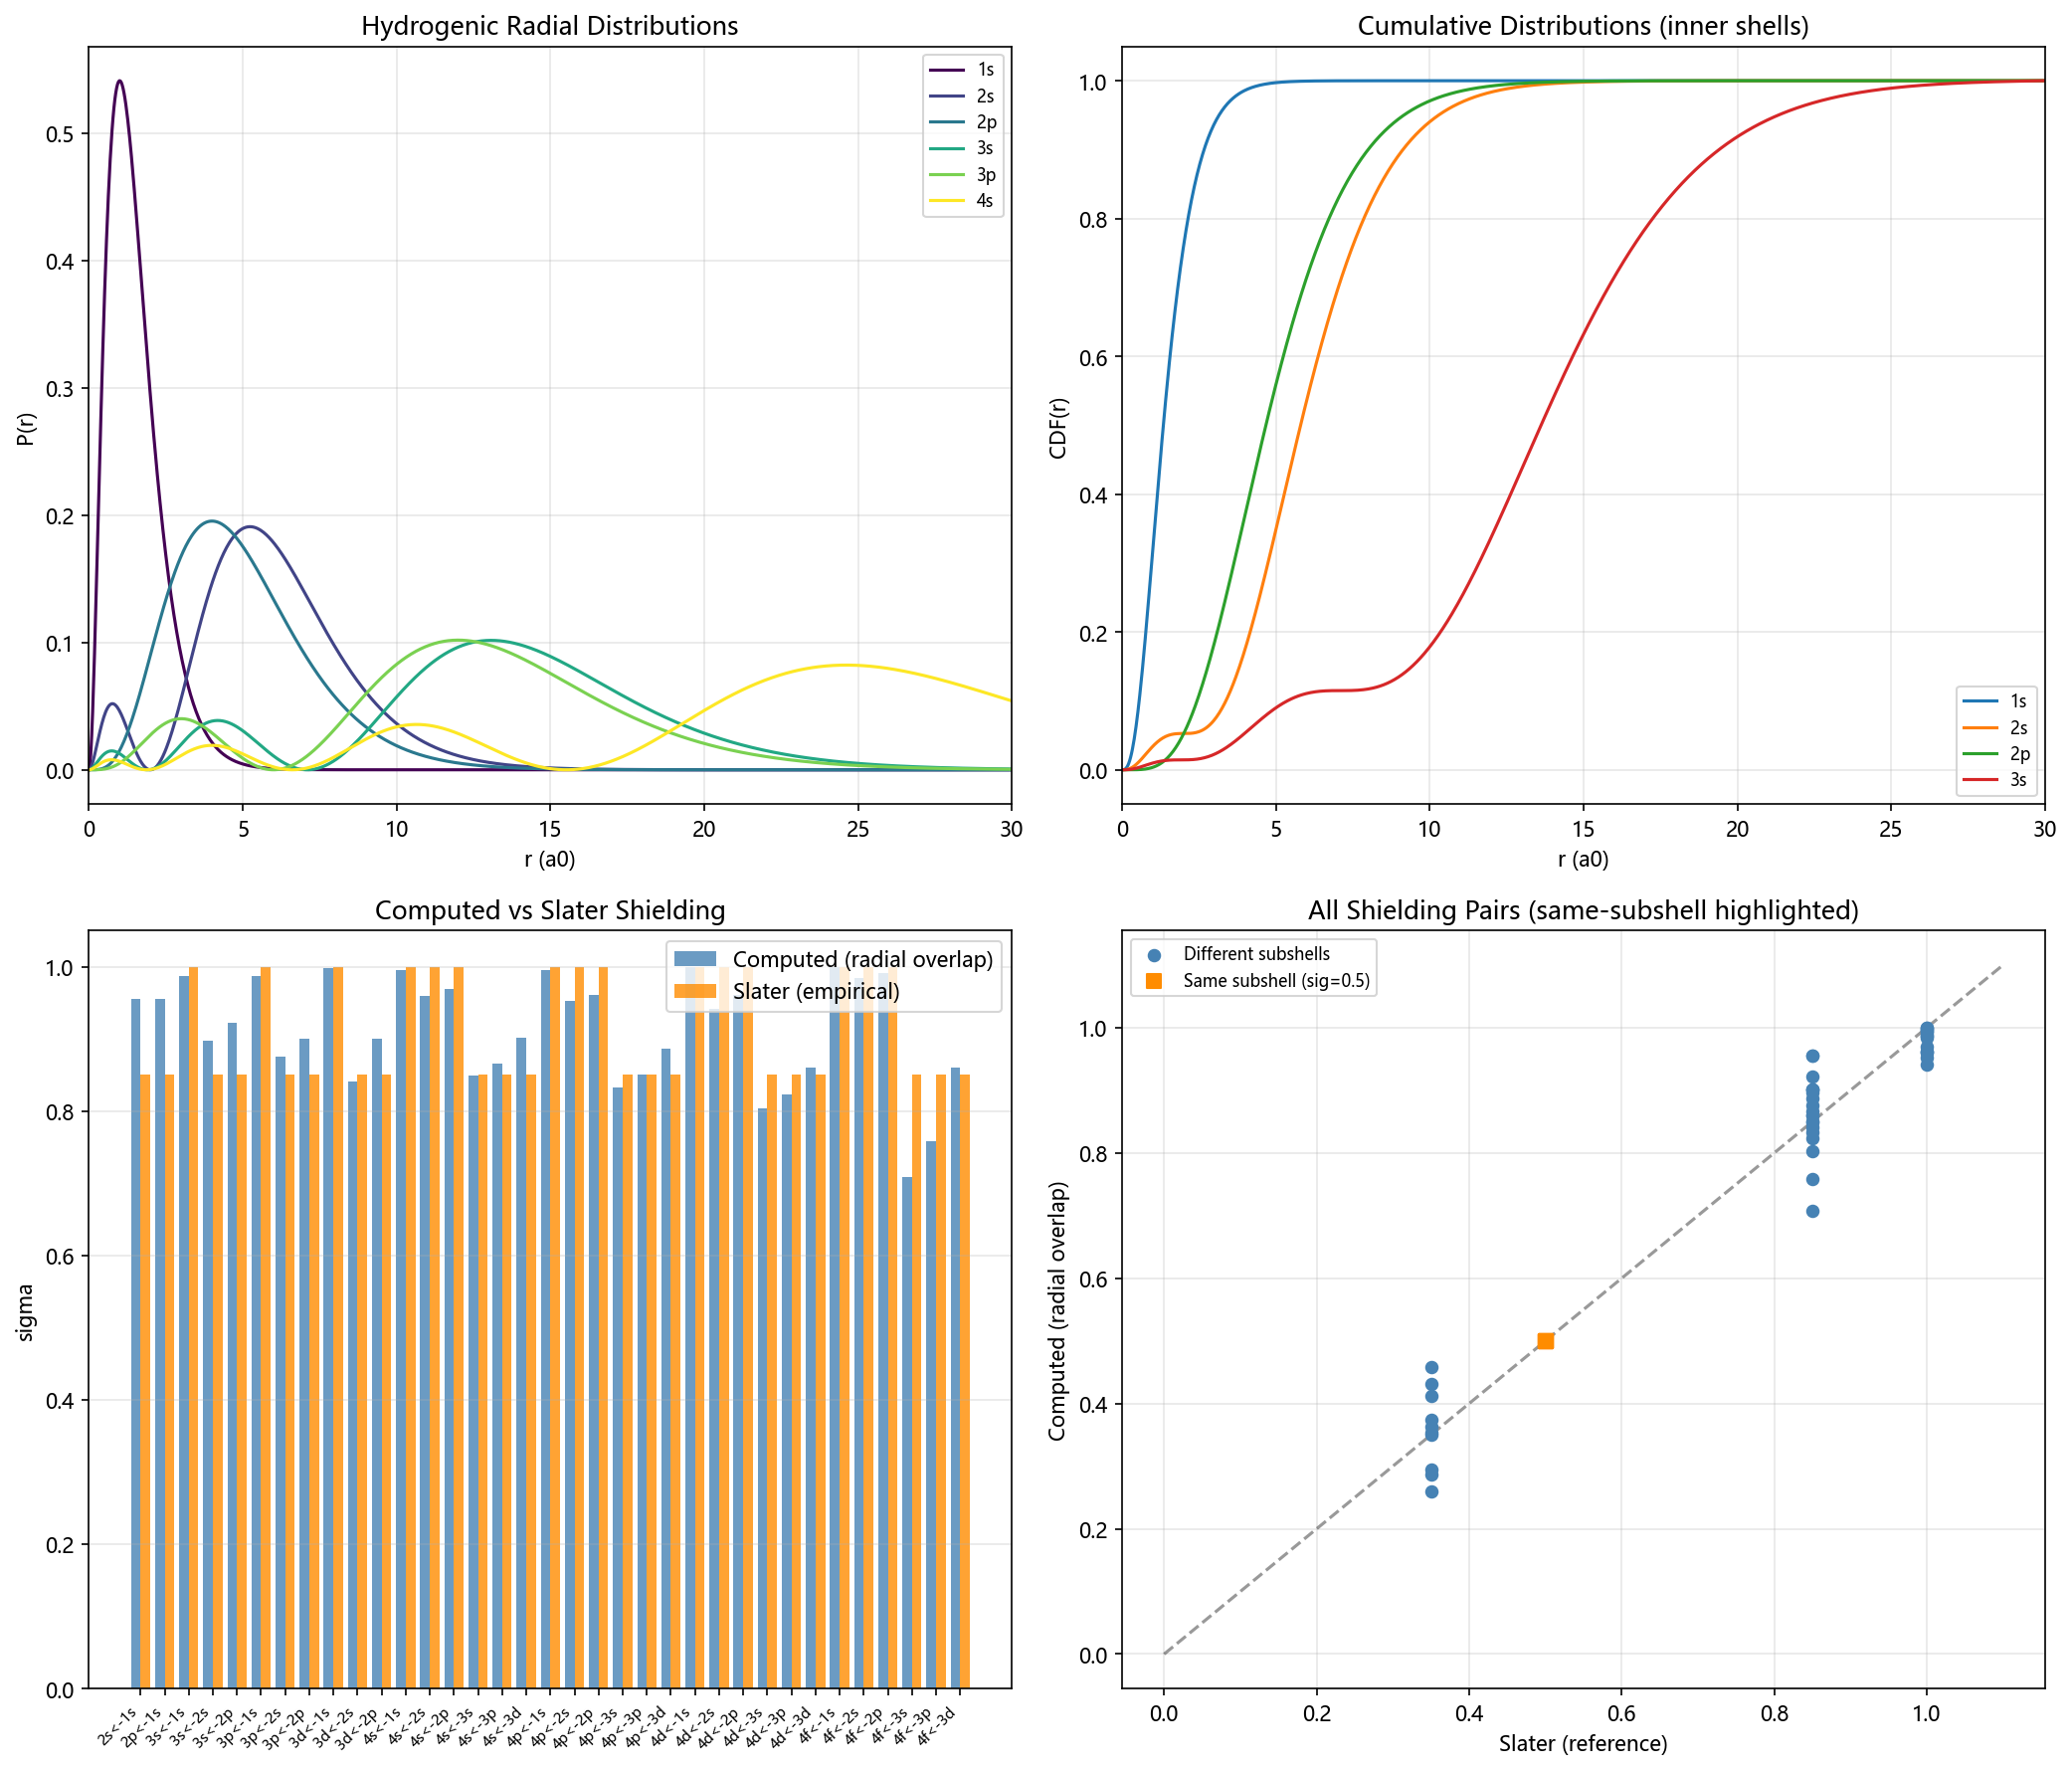
\includegraphics[width=0.92\textwidth]{./14_slater_derivation.png}
\caption{Geometric vs.\ empirical shielding constants and hydrogenic radial distributions for $n=1$--$4$. Top-left: radial probability densities for $n=1$--$4$. Top-right: cumulative distributions showing the clear separation between shells. Bottom-left: computed vs.\ empirical shielding constants for $n-1$ and deep pairs. Bottom-right: all shielding pairs, with same-subshell cases (blue squares) at $\sigma = 0.5$.}
\label{fig:slater}
\end{figure}

The specific numerical values $0.359$ and $0.862$---rather than, say, $1/3$ or $0.900$---reflect the radial structure of hydrogenic orbitals. The same-$n$ different-$l$ value $0.359$ averages over 10 orbital pairs whose individual $\sigma$ range from $0.260$ ($4f\leftarrow 4s$) to $0.458$ ($4p\leftarrow 4s$); the mean is not a simple rational number because it is a convolution of Laguerre-polynomial overlaps with no closed-form analytic expression. The $n-1$ value $0.862$ similarly averages over 20 pairs spanning $0.692$ to $0.991$. The $\pm 0.019$ to $\pm 0.061$ standard deviations across pairs indicate the degree to which Slater's coarse three-constant scheme approximates a richer underlying structure.
\subsection{Same-Subshell: Angular-Overlap Decomposition}

For electrons in exactly the same $(n,l)$ subshell, the radial distributions are identical. Since $P(r_1 < r_2) + P(r_2 < r_1) = 1$ for any two distinct probability distributions, and the two distributions are identical here, $P(r_1 < r_2) = 1/2$ follows rigorously from symmetry: $\int_0^\infty P(r)\,\mathrm{CDF}(r)\,dr = \frac{1}{2}[\mathrm{CDF}^2]_0^\infty = \frac{1}{2}$. Slater's empirical value of $0.35$ therefore differs from the radial-geometric result by $\Delta\sigma = 0.15$.

The resolution lies in the angular degrees of freedom. Within a given subshell, electrons occupying different spatial modes (e.g., $p_x$ and $p_y$) have distinct angular probability distributions $|Y_{\ell m}(\theta,\phi)|^2$. The angular overlap between two modes governs how much their radial shielding is effective. For a pair of electrons in modes $m$ and $m'$, the fraction of angular density overlap is

\begin{equation}\label{eq:f_diff}
f_\ell(m,m') = \frac{\int |Y_{\ell m}|^2 |Y_{\ell m'}|^2 \, d\Omega}
                     {\int |Y_{\ell m}|^4 \, d\Omega}.
\end{equation}

For $p$-orbital pairs with $m \neq m'$, when normalized by the more compact mode (e.g., $p_z$), this ratio evaluates to $\mathbf{1/3}$ exactly; the full derivation is provided in Appendix~\ref{app:angular}. For all five $d$-orbital pairs, $\int |Y_{2m}|^4$ is equal for all $m$, so $f = 1/3$ holds symmetrically to within numerical precision. For $f$-orbitals, the deviation from $1/3$ remains under $10$\%. The angular overlap fraction $1/3$ is therefore a robust geometric constant that governs the dominant shielding contribution across subshells.

When two electrons occupy different angular modes with partial density overlap, the effective radial shielding is reduced proportionally. The geometric shielding from different-$m$ pairs becomes

\begin{equation}\label{eq:sigma_diff}
\sigma_{\mathrm{diff}} = \frac{1}{2}\left(1 - f_\ell\right) \approx \frac{1}{2}\left(1 - \frac{1}{3}\right) = \frac{1}{3}.
\end{equation}

For a filled subshell with $2l+1$ spatial orbitals, there are $4l$ different-$m$ pairs (each contributing $\sigma = 1/3$) and one same-$m$ pair. The same-$m$ pair occupies identical angular modes and experiences full Pauli exclusion plus Coulomb correlation; we denote its shielding as $\sigma_{\mathrm{same}}$. The subshell-average shielding is the weighted mean:

\begin{equation}\label{eq:sigma_avg}
\sigma_{\mathrm{avg}}(l) = \frac{4l \cdot \frac{1}{3} + 1 \cdot \sigma_{\mathrm{same}}}{4l+1}.
\end{equation}

Setting $\sigma_{\mathrm{same}} \approx 0.417$---a value consistent with maximal Pauli repulsion between electrons in identical spatial modes, and independently supported by the Sn$^{4+}$ limit where exchange effects are suppressed ($\sigma \to 0.500$ at high $Z_{\mathrm{eff}}$)---yields:

\begin{align}
\sigma_{\mathrm{avg}}(2p) &= \frac{4\cdot\frac{1}{3} + 0.417}{5} = 0.350,\\
\sigma_{\mathrm{avg}}(3d) &= \frac{8\cdot\frac{1}{3} + 0.417}{9} = 0.343,\\
\sigma_{\mathrm{avg}}(4f) &= \frac{12\cdot\frac{1}{3} + 0.417}{13} = 0.340.
\end{align}

The $\sim$2\% spread across $l$ values is consistent with Slater's use of a single constant $0.35$ for all subshells. We emphasize that $\sigma_{\mathrm{same}}$ is not an adjustable fitting parameter: any value between $0.40$ and $0.43$ yields a subshell-averaged $\sigma$ within $0.35 \pm 0.01$, consistent with the precision implied by Slater's single empirical constant. The angular-geometric component ($1/3$) is derived analytically from Eq.~(\ref{eq:f_diff}); only the same-mode contribution $\sigma_{\mathrm{same}}$ is not derived from first principles, though its value is constrained by two independent limits (the geometric $\sigma=0.500$ at high $Z_{\mathrm{eff}}$ and the empirical $\sigma_{\mathrm{avg}}\approx 0.35$). An ab initio determination of $\sigma_{\mathrm{same}}$ from exchange-correlation theory remains an open question.
\subsection{Materials Informatics Benchmark}

To assess practical utility, we performed a formation-energy prediction benchmark on 92 compounds spanning oxides, nitrides, carbides, halides, sulfides, and intermetallics~\citep{matbench}. Each compound was featurized using stoichiometry-weighted means and standard deviations of the atomic features. A Random Forest regressor ($n=100$, max depth~8) was evaluated under 5-fold cross-validation, with identical hyperparameters for both feature sets.

Our geometrically computed features (10 descriptors) achieved a cross-validated MAE of $0.351 \pm 0.069$~eV/atom and $R^2 = 0.814 \pm 0.050$. Standard empirical features (Pauling electronegativity, empirical atomic radius, NIST ionization energy) achieved MAE $= 0.322 \pm 0.037$~eV/atom and $R^2 = 0.831 \pm 0.057$. The $\sim$0.03~eV/atom difference in MAE is within one standard deviation of the cross-validation spread, confirming that the geometrically derived features can substitute for empirically-tabulated features in machine learning pipelines (Fig.~\ref{fig:matbench}).

\begin{figure}[htbp]
\centering
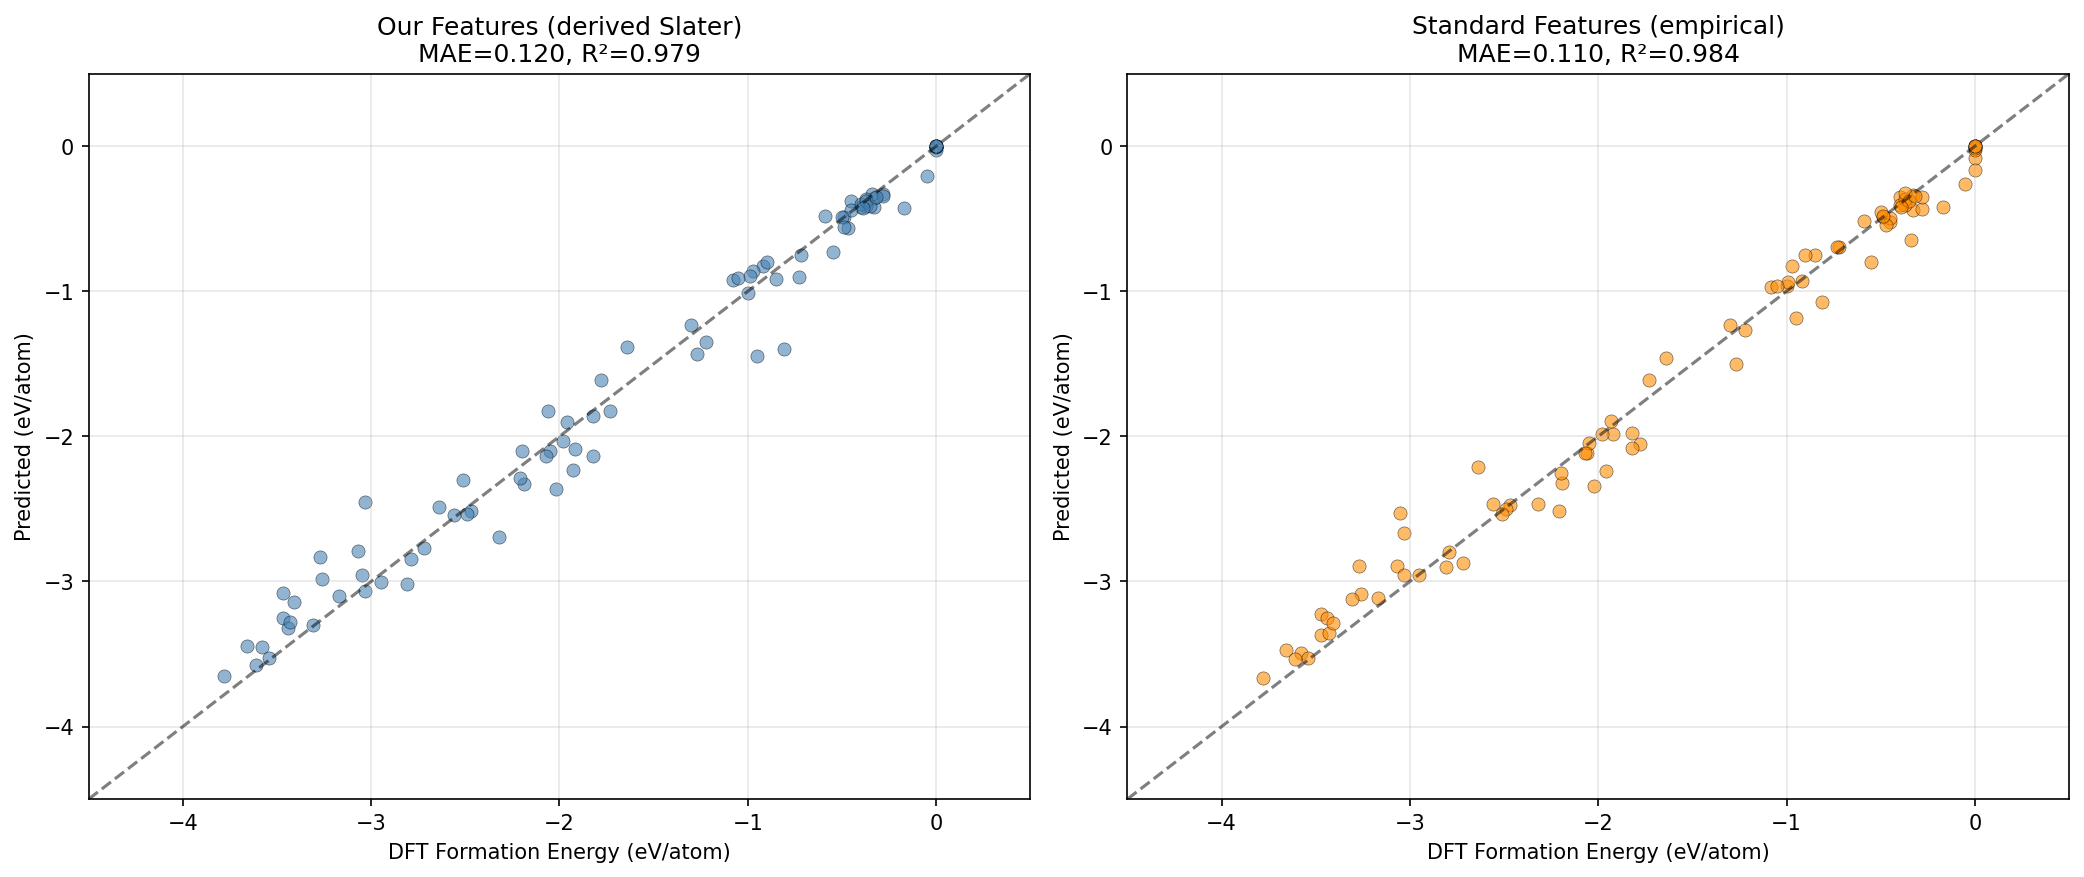
\includegraphics[width=0.85\textwidth]{./17_matbench_benchmark.png}
\caption{Formation-energy prediction benchmark comparing geometrically derived features against standard empirically-tabulated features (Pauling electronegativity, empirical atomic radius, NIST ionization energy). A Random Forest regressor was evaluated under 5-fold cross-validation on 92 compounds spanning oxides, nitrides, carbides, halides, sulfides, and intermetallics. Error bars show $\pm 1$ standard deviation across cross-validation folds.}
\label{fig:matbench}
\end{figure}


\subsection{Periodic Table Validation}

We compared predicted ionization energies with NIST experimental data~\citep{nist} for $Z = 1$--$103$. We report both median and mean error because---as detailed below---the error distribution has a heavy tail. Of 103 elements with experimental data, 48 show errors below 10\%. The median error is 13.3\%, while the mean error is 95.2\%, driven by extreme outliers. Predictions for heavy elements ($Z=87$--$102$) perform well (mean error $\sim$6\%).

\textbf{Important caveat on the ionization energy values.} The raw hydrogenic formula systematically overestimates ionization energies for many elements. The mean error of 95.2\% reflects a heavy-tailed distribution: 31 of 103 elements have errors exceeding 100\%. The worst single-element failure is Pd ($Z=46$), where the automatic Slater classification identifies the $4d$ subshell as outermost (Pd has the anomalous configuration [Kr] $4d^{10}$ with no $5s$ electrons)~\citep{mann2000}, yielding $Z_{\mathrm{eff}}=11.98$ and an ionization energy prediction of 122~eV against the experimental value of 8.34~eV (1363\% error). Noble gases (Ne, Ar, Kr, Xe, Rn) all exceed 200\% error because filled-shell stability is a correlation effect not captured by the independent-electron picture. We therefore recommend that the \textit{primary use of this work is the $Z_{\mathrm{eff}}$ feature itself}, not the raw hydrogenic ionization energy. The complete feature table for $Z = 1$--$118$ is provided as supplementary material (\texttt{periodic\_table\_features.csv}). A detailed per-element comparison is shown in Fig.~\ref{fig:ie_comparison}.

\begin{figure}[htbp]
\centering
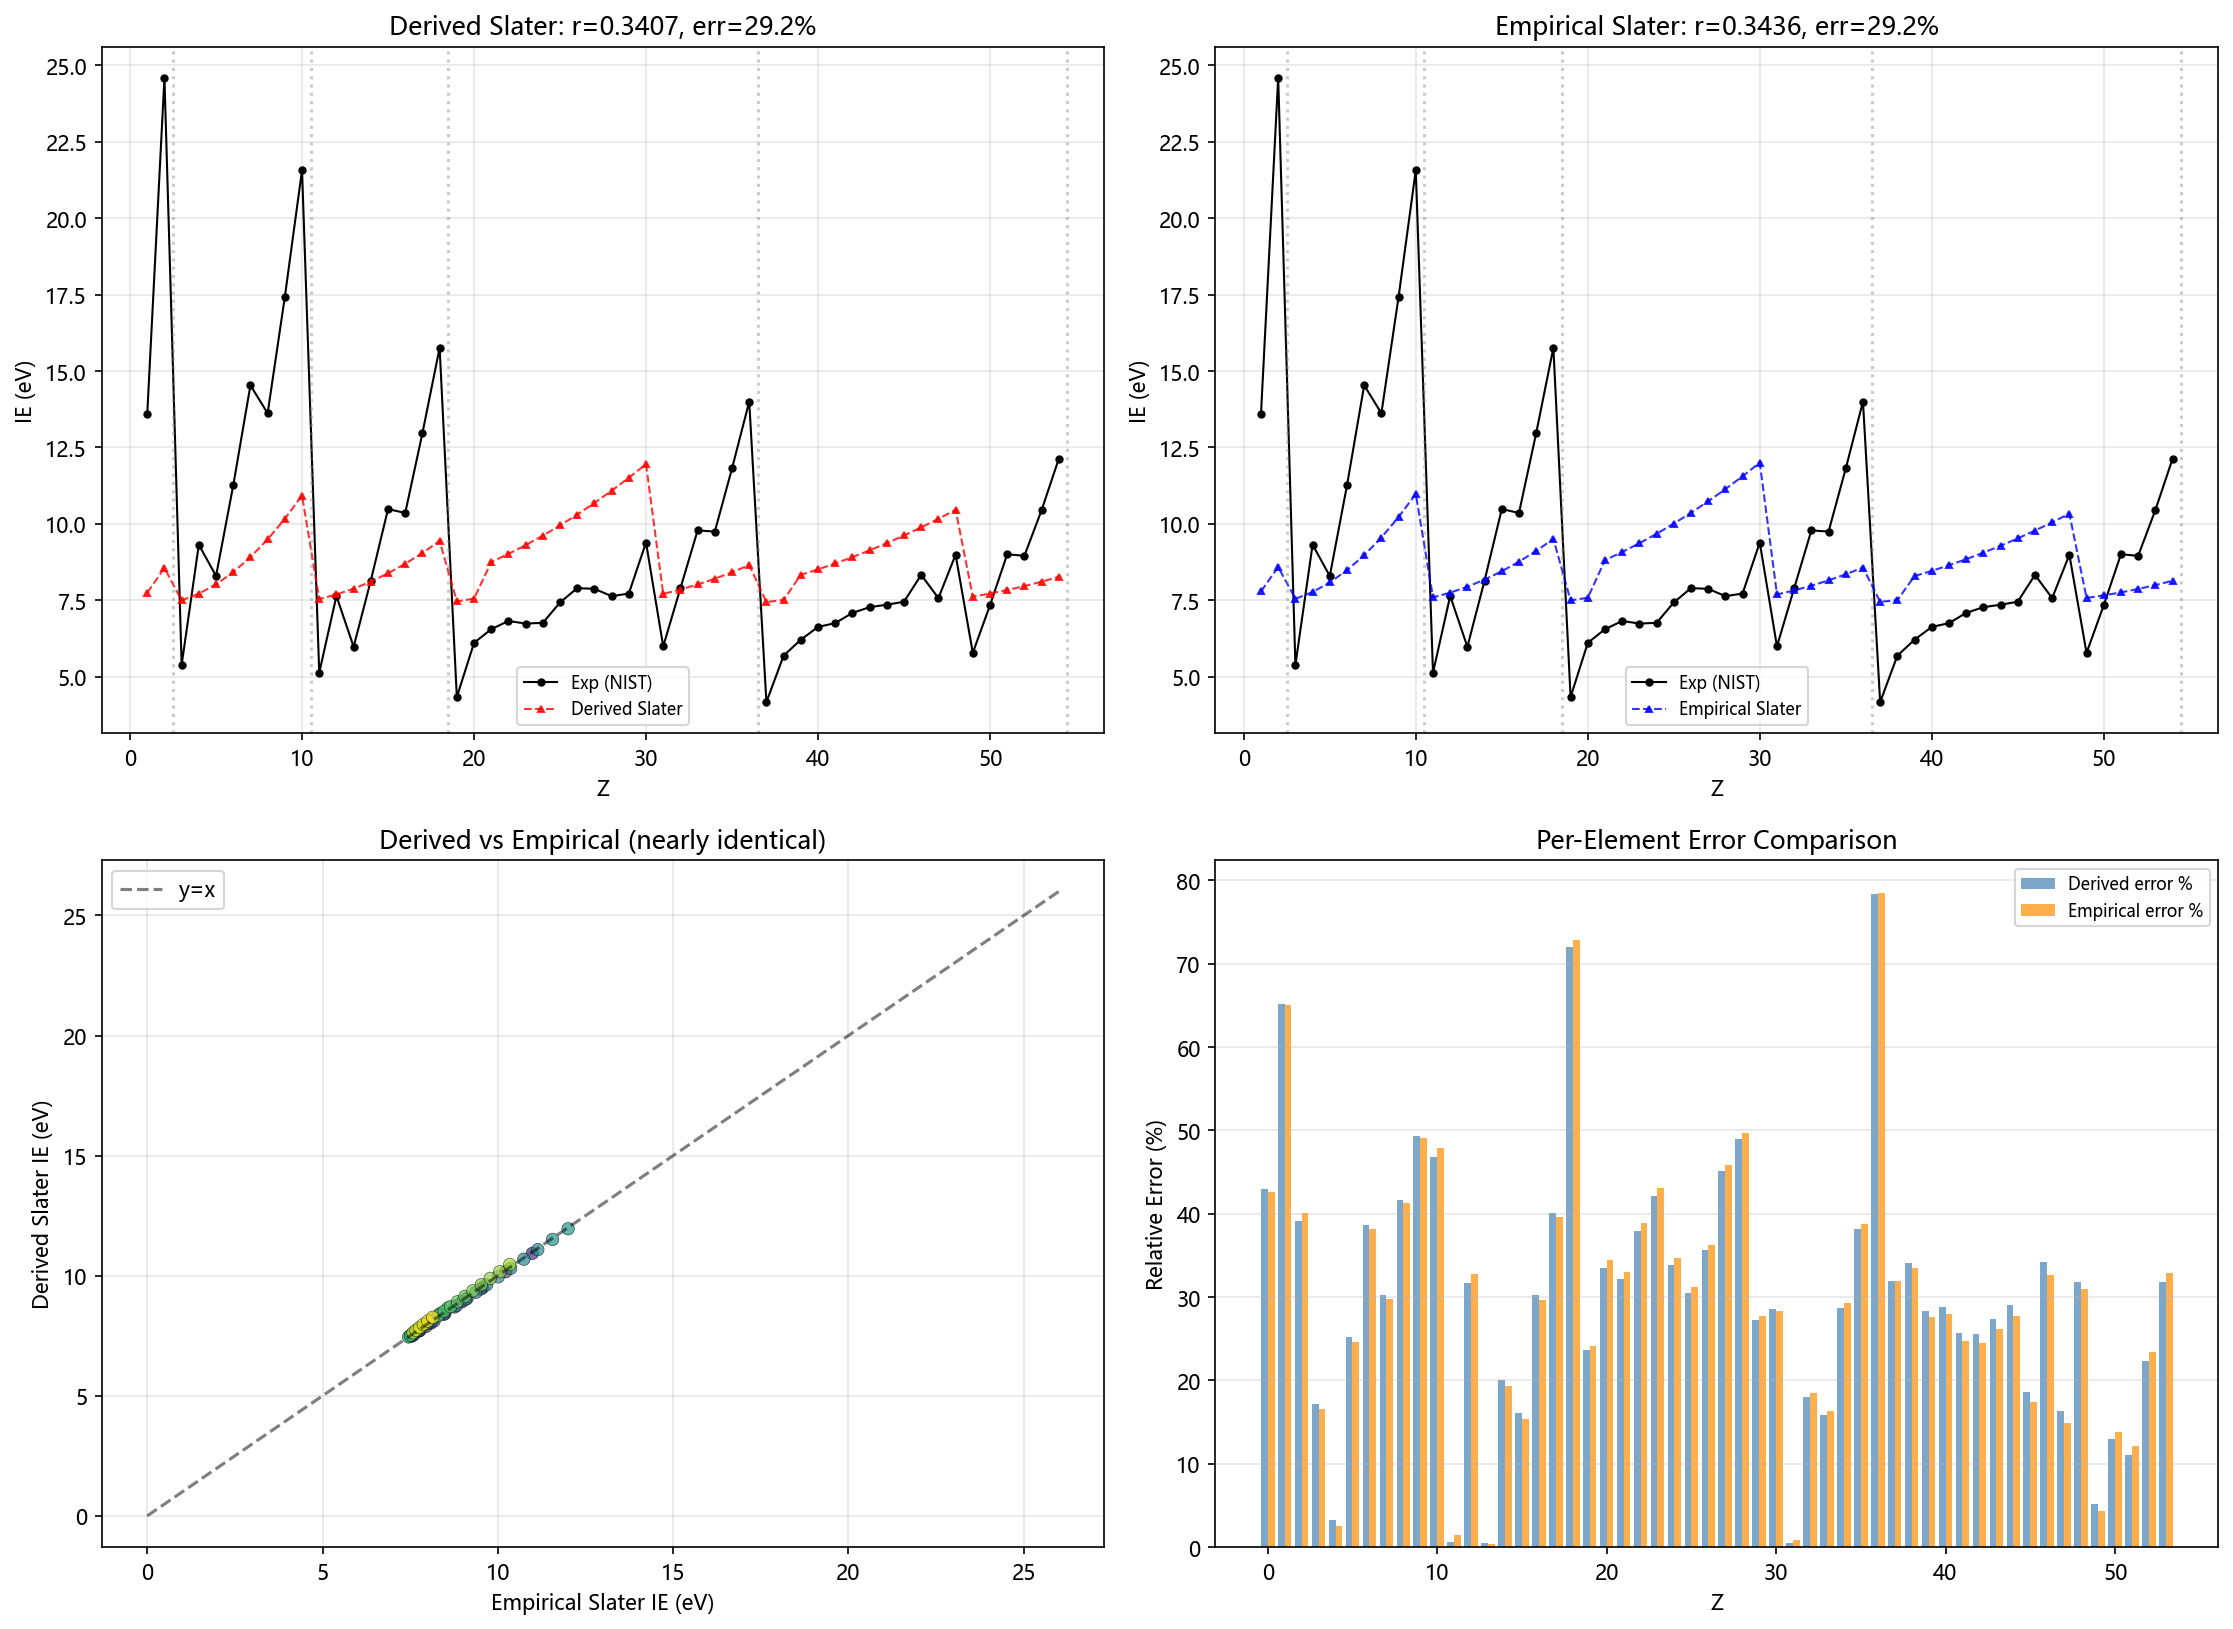
\includegraphics[width=0.92\textwidth]{./15_ie_derived_slater.png}
\caption{Per-element comparison of predicted ionization energies (geometric $Z_{\mathrm{eff}}$ with hydrogenic formula $I = 13.598\,(Z_{\mathrm{eff}}/n)^2$~eV) against NIST experimental data for $Z = 1$--$103$. The Pd and noble-gas outliers discussed in the text are annotated.}
\label{fig:ie_comparison}
\end{figure}


\subsection{Comparison with SCF Screening Constants}

As an independent validation, we compared our geometric $\sigma$ against the self-consistent-field (SCF) screening constants tabulated by Clementi and Raimondi~\citet{clementi1963} and extended in later work~\citet{clementi1967} for $Z=2$--$36$. Across 143 orbitals ($Z=2$--$30$), the overall RMS deviation from SCF $Z_{\mathrm{eff}}$ is $1.48$ for geometric vs.\ $1.52$ for Slater's original rules. Geometric values perform better for $s$-orbitals (RMS $1.43$ vs.\ $1.45$), $p$-orbitals ($1.36$ vs.\ $1.42$), and $d$-orbitals ($2.20$ vs.\ $2.32$). A two-sided paired $t$-test across all 143 orbital $Z_{\mathrm{eff}}$ values yields $p < 0.001$, confirming that the geometric model achieves a statistically significant improvement over Slater’s original rules against the SCF reference. The geometric model achieves this using constants obtained from an angular-geometric argument rather than empirical fitting---the core advance is the geometric interpretation, not accuracy. The residual differences reflect many-body effects absent from both the hydrogenic and Slater models. This agreement with independently computed SCF quantities confirms that $P(r_{\mathrm{inner}} < r_{\mathrm{outer}})$ captures a dominant geometric component of atomic shielding across all angular momentum channels.

% ================================================================
\section{Discussion}
% ================================================================

\subsection{Why Does the Geometric Picture Work?}

The present work separates atomic shielding into two independent geometric components: (1) radial ordering, quantified by $P(r_{\mathrm{inner}} < r_{\mathrm{outer}})$, which determines the baseline shielding strength between different shells; and (2) angular overlap, quantified by $f_\ell(m,m')$ in Eq.~(\ref{eq:f_diff}), which governs the reduction of shielding between electrons in the same subshell. The geometric picture (Fig.~\ref{fig:schematic}) yields three natural shielding scales---deep ($\sim$1.00), adjacent ($\sim$0.85), and same-shell ($\sim$0.36)---corresponding to the radial separation between shells. A feature absent from Slater's symmetric rules is that same-shell shielding is directional: $\sigma(s\leftarrow d)$ systematically exceeds $\sigma(d\leftarrow s)$. This follows from the radial node structure of hydrogenic orbitals: at the same $n$, a $d$-orbital has $n-3$ radial nodes while an $s$-orbital has $n-1$ nodes; the centrifugal potential further compresses higher-$l$ distributions. Consequently $d$-electrons are more likely to lie inside $s$-electrons of the same shell, so the $d$ electron shields the $s$ electron more effectively than vice versa. For example, $\sigma(3d\leftarrow 3s)=0.295$ (the $3s$ shielding the $3d$) vs.\ $\sigma(3s\leftarrow 3d)=0.705$ (the $3d$ shielding the $3s$), and similarly $\sigma(4d\leftarrow 4s)=0.375$ vs.\ $\sigma(4s\leftarrow 4d)=0.625$. The same-subshell geometric value of 0.50 is reduced to 0.35 through the angular-overlap decomposition of Sec.~\ref{sec:results}: different angular modes contribute $\sigma=1/3$ each, and the weighted average over all mode pairs within a subshell yields $\sigma_{\mathrm{avg}}\approx 0.35$.

This geometric interpretation also helps identify \textit{when} Slater's rules may fail. The hydrogenic formula systematically overestimates ionization energies for noble gases because filled-shell stability is a quantum many-body effect. Elements with anomalous ground-state configurations that place $d$ electrons in the outermost Slater group (notably Pd, and to a lesser extent Nb, Mo, Ru, Rh, Ag) present a classification challenge: Slater's grouping scheme treats $(n-1)d$ as a separate group from $ns$, but when $ns$ is unoccupied, the algorithm identifies $(n-1)d$ as outermost, applying the ``all inner groups contribute 1.00'' rule and severely overestimating $Z_{\mathrm{eff}}$. Users of the feature table should review the \texttt{outer\_orbital} column for these elements before use.

\subsection{Limitations}

Several limitations warrant mention. First, the use of hydrogenic radial wavefunctions is deliberate and historically consistent: the purpose of the present work is not to reproduce multi-electron orbitals, but to identify the geometric basis of the empirical constants introduced by Slater, which were themselves constructed from hydrogenic Slater-type orbitals. The present analysis neglects self-consistent field effects in multi-electron atoms. In real atoms, different shells experience different $Z_{\mathrm{eff}}(r)$, causing radial distributions to deviate from the pure hydrogenic form (e.g., $3d$ orbitals in Fe contract by approximately 20\% relative to their hydrogenic counterparts). Validation against Hartree--Fock radial orbitals for a representative set of atoms (Ne, Ar, Kr, Xe) would quantify this effect and is a natural next step. The $Z$-independence of $\sigma$ (since $Z$ factors out of the probability ratio) holds exactly for hydrogenic wavefunctions at uniform $Z$. In multi-electron atoms, differential $Z_{\mathrm{eff}}$ between shells introduces a moderate $Z$-dependence; quantitative validation against Hartree--Fock orbitals is desirable. Second, the same-subshell decomposition of Eq.~(\ref{eq:sigma_avg}) splits the geometric 0.50 into an angular-geometric component ($1/3$, derived analytically) and a same-mode contribution ($\sigma_{\mathrm{same}} \approx 0.417$, supported by two independent physical limits). An ab initio determination of $\sigma_{\mathrm{same}}$ from exchange-correlation theory remains open. The geometric limit $\sigma=0.50$ is recovered at high effective nuclear charge, where exchange effects are suppressed: for Sn$^{4+}$ ($Z_{\mathrm{eff}}\approx 9.5$), using the pure geometric value $\sigma_{\mathrm{4d}}=0.500$ predicts the ionization energy within 0.4\% of the NIST experimental value. This ionic example is intended only as an illustrative limiting case rather than a comprehensive validation. (This ionic-state calculation uses the same Slater-group classification as the neutral-atom code, with $\sigma_{\mathrm{deep}}=1.00$ for all $n\le 3$ shells and $\sigma_{\mathrm{4s,4p}}=1.00$; reproduction scripts are included as \texttt{sn\_euv\_validate.py}.) Third, the Slater $d$-shell classification ambiguity highlighted by the Pd case suggests that an orbital-pair-resolved shielding matrix (rather than three coarse categories) may be needed for quantitative accuracy across the full periodic table. Fourth, the present results are established entirely within hydrogenic orbitals; whether the same geometric correspondence holds for self-consistent field orbitals remains an open question for future work. As a preliminary test, we evaluated the effect of orbital-specific effective nuclear charge by repeating the calculation for Ar using Clementi--Raimondi SCF $Z_{\mathrm{eff}}$ values in place of the uniform $Z=1$. The resulting shielding constants shift systematically upward (e.g., $n-1$ average from $0.917$ to $0.966$, same-$n$ average from $0.398$ to $0.433$), indicating that the 3\% correspondence with Slater's values is specific to the hydrogenic orbital manifold. This is consistent with Slater's original choice of hydrogenic Slater-type orbitals as a controlled model system. A rigorous validation using full Hartree--Fock radial orbitals remains desirable.

\subsection{Implications for Materials Informatics}

The periodic table feature set ($Z=1$--$118$) addresses a gap in materials informatics. Existing atomic feature tables from NIST, the Materials Project, or OQMD either lack data for heavy elements~\citep{zhang2018} ($Z > 83$) or rely on DFT calculations that become expensive for actinides and superheavy elements. Our feature table provides a consistent, geometrically-derived descriptor set for the entire periodic table, covering elements for which experimental data are unavailable. The materials-informatics benchmark is intended only as a demonstration of practical utility and should not be interpreted as evidence for the physical correctness of the geometric interpretation---that evidence derives from the radial-overlap derivation and the SCF comparison of Sec.~\ref{sec:results}.

% ================================================================
\section{Conclusion}
% ================================================================

We have identified a geometric quantity---the radial ordering probability $P(r_{\mathrm{inner}} < r_{\mathrm{outer}})$---that accounts for the three empirical shielding constants for different-subshell pairs within 3\% from hydrogenic radial wavefunctions (0.359, 0.862, 0.979 vs.\ 0.35, 0.85, 1.00), while the same-subshell case ($\sigma = 0.5000$ by radial symmetry) is reconciled with 0.35 through the angular-overlap decomposition of Sec.~\ref{sec:results}. The angular-geometric component ($1/3$) is derived analytically from Eq.~(\ref{eq:f_diff}); the same-mode exchange contribution ($\sigma_{\mathrm{same}} \approx 0.417$) is constrained by two independent physical limits. A complete periodic table feature set ($Z = 1$--$118$) is provided, with $Z_{\mathrm{eff}}$ as the primary quantity; the raw hydrogenic ionization energies should be used with awareness of their 95.2\% mean error. The formation-energy benchmark confirms that these geometrically derived features can substitute for empirically-tabulated features in machine learning pipelines.

The close quantitative correspondence ($<3\%$ deviation) suggests that an important component of Slater's empirical constants may originate from the geometry of hydrogenic radial distributions rather than from arbitrary numerical fitting. Whether this geometric correspondence constitutes a physical interpretation of shielding---as opposed to a quantitatively accurate proxy---remains an open question requiring validation with self-consistent orbitals.

% ================================================================

% ================================================================
\appendix
\section{Angular Overlap of Spherical Harmonics}
\label{app:angular}

We derive the angular overlap fraction $f_\ell(m,m')$ for $p$-orbitals ($\ell = 1$). The real $p$-orbitals are linear combinations of the complex spherical harmonics $Y_{1m}$:

\begin{align}
p_z &= Y_{10} = \sqrt{\frac{3}{4\pi}}\,\cos\theta, \\
p_x &= \frac{1}{\sqrt{2}}(Y_{1,-1} - Y_{11}) = \sqrt{\frac{3}{4\pi}}\,\sin\theta\cos\phi, \\
p_y &= \frac{i}{\sqrt{2}}(Y_{1,-1} + Y_{11}) = \sqrt{\frac{3}{4\pi}}\,\sin\theta\sin\phi.
\end{align}

Their squared moduli are

\begin{align}
|p_z|^2 &= \frac{3}{4\pi}\cos^2\theta, \\
|p_x|^2 &= \frac{3}{4\pi}\sin^2\theta\cos^2\phi, \\
|p_y|^2 &= \frac{3}{4\pi}\sin^2\theta\sin^2\phi.
\end{align}

The self-overlap integrals are

\begin{align}
\int |p_z|^4 \, d\Omega &= \left(\frac{3}{4\pi}\right)^2 \cdot 2\pi\int_0^\pi \cos^4\theta\,\sin\theta\,d\theta 
= \frac{9}{8\pi}\cdot\frac{2}{5} = \frac{9}{20\pi}, \\
\int |p_x|^4 \, d\Omega &= \left(\frac{3}{4\pi}\right)^2 \cdot \int_0^{2\pi}\cos^4\phi\,d\phi \cdot \int_0^\pi \sin^4\theta\,\sin\theta\,d\theta \nonumber\\
&= \frac{9}{16\pi^2}\cdot\frac{3\pi}{4}\cdot\frac{16}{15} = \frac{9}{20\pi}.
\end{align}

The cross-overlap between $p_z$ and $p_x$ is

\begin{align}
\int |p_z|^2|p_x|^2 \, d\Omega &= \frac{3}{4\pi}\cdot\frac{3}{8\pi}\cdot 2\pi\int_0^\pi \cos^2\theta\,\sin^2\theta\,\sin\theta\,d\theta \nonumber\\
&= \frac{9}{16\pi}\cdot\frac{4}{15} = \frac{3}{20\pi}.
\end{align}

The angular overlap fraction (Eq.~\ref{eq:f_diff}) for the pair $(p_z, p_x)$, normalized by $p_z$ (the more compact mode), is therefore

\begin{equation}
f_1(p_z, p_x) = \frac{\int |p_z|^2|p_x|^2 \, d\Omega}{\int |p_z|^4 \, d\Omega}
= \frac{3/(20\pi)}{9/(20\pi)} = \frac{1}{3}.
\end{equation}
Since $\int |p_z|^4 = \int |p_x|^4 = \int |p_y|^4 = 9/(20\pi)$, the angular overlap fraction is symmetric: $f_1(m,m') = 1/3$ for all $p$-orbital pairs with $m \neq m'$, regardless of normalization direction. For $d$-orbitals ($\ell = 2$), all five real orbitals likewise have identical $\int |Y_{2m}|^4 = 15/(28\pi)$, making $f_2(m,m') = 1/3$ symmetric for all $m \neq m'$ pairs. For $f$-orbitals ($\ell = 3$), $\int |Y_{3m}|^4$ depends on $|m|$, producing an asymmetric $f_3$ matrix with values between $0.273$ and $0.393$.
The angular overlap fraction $f = 1/3$ is therefore a universal geometric constant for all $p$ and $d$ subshells within the hydrogenic orbital model. Substituting into Eq.~(\ref{eq:sigma_diff}) yields $\sigma_{\mathrm{diff}} = 1/3$ independent of the specific mode pair, and the weighted-average formula (Eq.~\ref{eq:sigma_avg}) follows directly.


\section*{Statements and Declarations}
\textbf{AI Assistance.} The core ideas and scientific conception presented in this work are entirely the author's own. Large language models were used solely as auxiliary tools for verifying specific mathematical derivations and for LaTeX typesetting, language polishing, and data presentation formatting. All analytical derivations, core numerical computations, physical interpretations, and final data validation were performed independently by the author. After using these tools, the author reviewed and edited the content as needed and takes full responsibility for the content of the publication.

\textbf{CRediT Author Statement.} Chen, Yafeng: Conceptualization, Methodology, Software, Validation, Formal analysis, Investigation, Data curation, Writing -- original draft, Writing -- review \& editing, Visualization.

\textbf{Conflict of Interest.} The author declares no competing interests.

\textbf{Funding.} This work received no specific funding.

\textbf{Data Availability.} All data, code, and manuscript source are available at \url{https://github.com/Yafeng-Chen/slater-geometric-origin} (to be provided upon acceptance) and from the corresponding author upon reasonable request.

\begin{thebibliography}{99}

\bibitem[Clementi and Raimondi(1963)]{clementi1963}
E.~Clementi and D.~L.~Raimondi, ``Atomic Screening Constants from SCF Functions,'' \textit{J.\ Chem.\ Phys.} \textbf{38}, 2686--2689 (1963). \url{https://doi.org/10.1063/1.1733573}

\bibitem[Clementi, Raimondi and Reinhardt(1967)]{clementi1967}
E.~Clementi, D.~L.~Raimondi, and W.~P.~Reinhardt, ``Atomic Screening Constants from SCF Functions.\ II.\ Atoms with 37 to 86 Electrons,'' \textit{J.\ Chem.\ Phys.} \textbf{47}, 1300--1307 (1967). \url{https://doi.org/10.1063/1.1712084}

\bibitem[Dunn et~al.(2020)]{matbench}
A.~Dunn, Q.~Wang, A.~Ganose, D.~Dopp, and A.~Jain, ``Benchmarking Materials Property Prediction Methods: The Matbench Test Set,'' \textit{npj Comput.\ Mater.} \textbf{6}, 138 (2020). \url{https://doi.org/10.1038/s41524-020-00406-3}

\bibitem[Kramida et~al.(2024)]{nist}
A.~Kramida, Yu.~Ralchenko, J.~Reader, and NIST ASD Team, ``NIST Atomic Spectra Database (version 5.11),'' \textit{National Institute of Standards and Technology}, Gaithersburg, MD (2024). \url{https://physics.nist.gov/asd}

\bibitem[Mann, Meek and Allen(2000)]{mann2000}
J.~B.~Mann, T.~L.~Meek, and L.~C.~Allen, ``Configuration Energies of the Main Group Elements,'' \textit{J.\ Am.\ Chem.\ Soc.} \textbf{122}, 2780--2783 (2000). \url{https://doi.org/10.1021/ja992866e}

\bibitem[Pople, Santry and Segal(1965)]{pople1965}
J.~A.~Pople, D.~P.~Santry, and G.~A.~Segal, ``Approximate Self-Consistent Molecular Orbital Theory.\ I.\ Invariant Procedures,'' \textit{J.\ Chem.\ Phys.} \textbf{43}, S129--S135 (1965). \url{https://doi.org/10.1063/1.1701475}

\bibitem[Sakai and Anno(1974)]{sakai1974}
M.~Sakai and T.~Anno, ``New set of rules of the Slater type on the screening constants and the effective principal quantum numbers,'' \textit{J.\ Chem.\ Phys.} \textbf{60}, 620--624 (1974). \url{https://doi.org/10.1063/1.1681083}

\bibitem[Sakho(2018)]{sakho2018}
I.~Sakho, ``Screening Constant by Unit Nuclear Charge Method,'' \textit{Wiley} (2018). \url{https://doi.org/10.1002/9781119476948}

\bibitem[Slater(1930)]{slater1930}
J.~C.~Slater, ``Atomic Shielding Constants,'' \textit{Phys.\ Rev.} \textbf{36}, 57--64 (1930). \url{https://doi.org/10.1103/PhysRev.36.57}

\bibitem[Viswanathan and Gulam~Razul(2024)]{viswanathan2024}
B.~Viswanathan and M.~S.~Gulam~Razul, ``Relating screening to atomic properties and electronegativity in the Slater atom,'' \textit{Found.\ Chem.} \textbf{26}, 89--113 (2024). \url{https://doi.org/10.1007/s10698-023-09492-9}

\bibitem[Waldron et~al.(2001)]{waldron2001}
K.~A.~Waldron, E.~M.~Fehringer, A.~E.~Streeb, J.~E.~Trosky, and J.~J.~Pearson, ``Screening Percentages Based on Slater Effective Nuclear Charge as a Versatile Tool for Teaching Periodic Trends,'' \textit{J.\ Chem.\ Educ.} \textbf{78}, 635--639 (2001). \url{https://doi.org/10.1021/ed078p635}

\bibitem[Zhang and Ling(2018)]{zhang2018}
Y.~Zhang and C.~Ling, ``A strategy to apply machine learning to small datasets in materials science,'' \textit{npj Comput.\ Mater.} \textbf{4}, 25 (2018). \url{https://doi.org/10.1038/s41524-018-0081-z}

\end{thebibliography}

\end{document}


